\chapter{\lookout}
\label{cha:lookout}
\section{Linux Kernel}\label{sec:kernel}
Das Git Repository des Linux Kernels wurde am 16 April 2005 initial von Linus
Torvalds mit folgendem \gls{commit}\cite{link:linuxgit} eröffnet:

\lstinputlisting[
  label=lst:linusfirst,
  caption={Erster Git Commit von Linus Torvalds},
  frame=L,
  numbers=none,
  basicstyle=\footnotesize,
]{listings/linus_first_git_commit.lst}

Der Linux Kernel ist eines der populärsten Git Repositorys und unterstreicht
die technischen Möglichkeiten von Git mit einigen, durchaus beindruckenden,
Statistiken.

Seid der Version (\textit{2.6.12-rc2}) vom 16 April 2005 ist der Inhalt des
\glspl{repository} auf insgesamt 61.287 Dateien mit 17.734.793 Zeilen Quellcode
angewachsen. In dem Zeitraum zwischen 2005 und 2017 haben 17.225 verschiedene
Autoren in 693.782 Commits 36.122.715 Zeilen Quellcode hinzugefügt und
18.387.922 entfernt. Das sind ca. 40 Commits pro Author und durchschnittlich
157 Commits am Tag. Das Repository enthält ca. 530 versionierte \glspl{tag}
mit durchschnittlich 1309 Commits pro \glspl{tag}(bzw. Version). Insgesamt wurden
51.667 Merges durchgeführt von denen Linus Torvalds 22.043 selbst durchgeführt
hat. Abbildung \ref{top20} gibt einen Überblick der 20 Autoren die diese
Statistiken anführen.

\begin{figure}
	\centering
  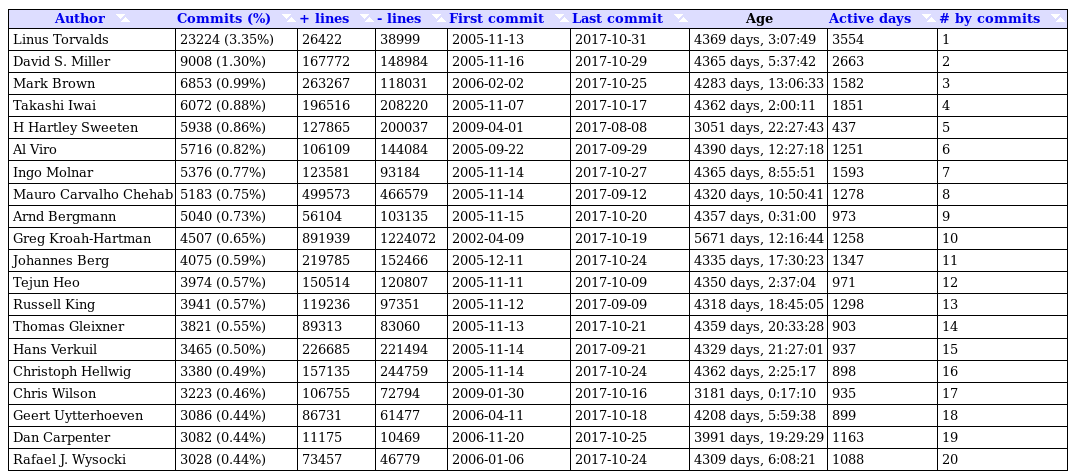
\includegraphics[scale=0.40]{images/top_20_of_linux_authors.png}
	\caption{Top 20 Linux Kernel Autoren}
	\label{top20}
\end{figure}

Diese Statistiken wurden entweder mit gitstats\cite{link:gitstats} und standard
Git Befehlen ermittelt. So lassen sich z.B. unter Linux die durchgeführten
Merges von Linus Torvalds mit folgendem Befehl ermitteln:

\lstinputlisting[
  label=lst:allmerges,
  caption={Ermitteln von Merges pro Autor},
  frame=none,
  numbers=none,
  basicstyle=\footnotesize,
]{listings/all_merges.lst}

Statistiken wie o.a. sind aber nicht unbedingt als Qualitätsmaßstab geeignet um
Rückschlüsse auf die Effizienz einzelner Personen zu ziehen.  Wie in Kapitel
\ref{sec:collaboration} beschrieben sollten diese Informationen aber trotzdem
allen Beteiligten zur Verfügung gestellt werden.  So wird nach Jez Humble und
David Farley in \cite[S.~138]{cd} eine Messung der geschriebenen Zeilen
Quellcode am Tag warscheinlich eher dazu führen das Entwickler kürzere Zeilen
Quellcode als effizientere schreiben. Die gemessene Anzahl an Commits hingegen
evtl. dazu das Änderungen pro Commit kleiner werden und dadurch besser
nachvollziehbar.

Es können verschiedenste Statistiken über das Projekt erhoben werden.
Beispielsweise könnten das nach Jez Humble und David Farley in
\cite[S.~138]{cd}folgende sein:

\begin{itemize}
\item Testabdeckung,
\item Anzahl der Fehler,
\item Anzahl der \glspl{commit},
\item Anzahl der fehlgeschlagenen/erfolgreichen Versuche die Software zu erstellen,
\item Metriken über den Quellcode (Zyklen, Duplikate o.a.),
\end{itemize}


\section{Git in Unternehmen und Projekten}
\section{Git im Internet}
\section{Statistiken}
\chapter{\result}\label{cha:result}

\chapter{Notizen}
Use Meaningful commit Messages cd S. 37
Version Control: The Freedom to Delete cd S. 35
No binaries in VCS S.35 top
